\documentclass[a4paper,9pt]{beamer}\usepackage[]{graphicx}\usepackage[]{color}
%% maxwidth is the original width if it is less than linewidth
%% otherwise use linewidth (to make sure the graphics do not exceed the margin)
\makeatletter
\def\maxwidth{ %
  \ifdim\Gin@nat@width>\linewidth
    \linewidth
  \else
    \Gin@nat@width
  \fi
}
\makeatother

\definecolor{fgcolor}{rgb}{0.345, 0.345, 0.345}
\newcommand{\hlnum}[1]{\textcolor[rgb]{0.686,0.059,0.569}{#1}}%
\newcommand{\hlstr}[1]{\textcolor[rgb]{0.192,0.494,0.8}{#1}}%
\newcommand{\hlcom}[1]{\textcolor[rgb]{0.678,0.584,0.686}{\textit{#1}}}%
\newcommand{\hlopt}[1]{\textcolor[rgb]{0,0,0}{#1}}%
\newcommand{\hlstd}[1]{\textcolor[rgb]{0.345,0.345,0.345}{#1}}%
\newcommand{\hlkwa}[1]{\textcolor[rgb]{0.161,0.373,0.58}{\textbf{#1}}}%
\newcommand{\hlkwb}[1]{\textcolor[rgb]{0.69,0.353,0.396}{#1}}%
\newcommand{\hlkwc}[1]{\textcolor[rgb]{0.333,0.667,0.333}{#1}}%
\newcommand{\hlkwd}[1]{\textcolor[rgb]{0.737,0.353,0.396}{\textbf{#1}}}%
\let\hlipl\hlkwb

\usepackage{framed}
\makeatletter
\newenvironment{kframe}{%
 \def\at@end@of@kframe{}%
 \ifinner\ifhmode%
  \def\at@end@of@kframe{\end{minipage}}%
  \begin{minipage}{\columnwidth}%
 \fi\fi%
 \def\FrameCommand##1{\hskip\@totalleftmargin \hskip-\fboxsep
 \colorbox{shadecolor}{##1}\hskip-\fboxsep
     % There is no \\@totalrightmargin, so:
     \hskip-\linewidth \hskip-\@totalleftmargin \hskip\columnwidth}%
 \MakeFramed {\advance\hsize-\width
   \@totalleftmargin\z@ \linewidth\hsize
   \@setminipage}}%
 {\par\unskip\endMakeFramed%
 \at@end@of@kframe}
\makeatother

\definecolor{shadecolor}{rgb}{.97, .97, .97}
\definecolor{messagecolor}{rgb}{0, 0, 0}
\definecolor{warningcolor}{rgb}{1, 0, 1}
\definecolor{errorcolor}{rgb}{1, 0, 0}
\newenvironment{knitrout}{}{} % an empty environment to be redefined in TeX

\usepackage{alltt}
%

 \mode<presentation>
{
  \usetheme{Singapore}      % or try Darmstadt, Madrid, Warsaw, ...
  \usecolortheme{} % or try albatross, beaver, crane, ...
  \usefonttheme{serif}  % or try serif, structurebold, ...
  \mode<presentation>{\useinnertheme{rounded}}
  \setbeamertemplate{navigation symbols}{}
  \setbeamertemplate{caption}[numbered]
  \addtobeamertemplate{navigation symbols}{}{%
    \usebeamerfont{footline}%
    \usebeamercolor[fg]{footline}%
    \hspace{1em}%
    %\insertfrawas done by one doctor menumber/\inserttotalframenumber
}
} 
\usepackage{float}
\usepackage{graphicx}
\usepackage{mathtools}
\usepackage{amsmath}
\usepackage[english]{babel}
\usepackage[utf8x]{inputenc}
\usepackage{color, colortbl}
\usepackage{subfig}
\usepackage{listings}
\title{Results so Far(Univariate Analysis)}

\author{Olusoji Oluwafemi Daniel (1541893)}
\institute{Hasselt University, Belgium}
\date{\today}
\IfFileExists{upquote.sty}{\usepackage{upquote}}{}
\begin{document}
\begin{frame}
\titlepage
%\includegraphics[width=25mm]{1.png}
\end{frame}

\begin{frame}{Contents}
\tableofcontents
\end{frame}

\section{Introduction}
\begin{frame}{Background \& Objectives}
\tiny
\begin{block}{Background}
\begin{itemize}
\item The human microbiome is made up of trillions of symbiotic bacteria cells in humans(Ursell, et al, 2013).
\item Although their functions is not yet fully understood, they are associated with nutrition, metabolism, immune function and human physiology(Bull \& Plummer, 2013).
\item The part of the human microbiome that reside in the gastrointestinal tract(GUT) are even associated with more functions than others(Bull \& Plummer, 2013).
\item Changes in the GUT microbiome have been associated with; obesity, lipid accumulation and metabolic disorder(Boulange, et al, 2016). 
\item However, the exact causal relationships between this microbiome ecosystem and health conditions is not yet fully understood due to the complex pathology involved(Boulange, et al, 2016).
\item These established associations are however enough to trigger scientists and pharmaceutical establishments to develop treatments that target these microbiome ecosystem, to trigger a benefitial treatment effect in patients with associated health disorders.
\item But if this is to be achieved, elements of the GUT microbiome must be tied to health benefits in these patients, hence they must be good surrogates for already established measures of treatment effect in these patients(e.g., insulin sensitivity).
\end{itemize}
\end{block}

\begin{block}{Objectives}
The main objective of this thesis is to discover bacterias in gut microbiome that can serve as surrogate for insulin sensitivity in patients with metabolic syndrome.  Specifically;
\begin{itemize}
\item it is of interest to examine each of 30 candidates as a potential surrogate for insulin sensitivity,
\item Identify a combination of these 30 that can be a surrogate for insulin sensitivity.
\end{itemize}
\end{block}
\end{frame}

\begin{frame}{Notations for Response, Surrogates and Treatment}
\begin{itemize}
\item $\mathbf{T_i}$ = difference in insulin sensitivity, which is the true endpoint, $i=1,\ldots,16$
\item $\mathbf{S_{ij}}$ = surrogates (difference in bacteria counts),  $j=1,\ldots,30$. 
\item $\mathbf{X_i}$ = Treatment applied. own\_feces(control), donor\_feces(experimental).
\item C=control treatment and E=Experimental treatment
\end{itemize}

\end{frame}

\section{Methods}
\begin{frame}{Joint Modelling Approach(JMA)}
\begin{itemize}
\item The joint model framework to surrogate evaluation (Molenberghs, Burzykowski, Renard and Geys, 2000, Burzykowski, Molenberghs, and Buyse, 2005,  Buyse, et al, 2015, Perualia-Tan, et al, 2016) can be extended to the following surrogate specific joint model;
$$ \left( \begin{array}{c}
S_{ij} \\
T_{i}
\end{array} \right) \sim N\left[ \left( \begin{array}{c}
\mu_{S} + \alpha_jX_i  \\
\mu_{T} + \beta X_i
\end{array}
\right), \Sigma_j \right], \Sigma_j = \left( \begin{array}{cc}
\sigma_{SS} & \sigma_{ST}\\
\sigma_{ST} & \sigma_{TT}
\end{array}\right)$$

\item $\alpha_j$ is the effect of treatment on surrogate j 
\item $\beta$ is the effect of treatment on the true endpoint
\item $\rho_{T,S|X} = \frac{\sigma_{ST}}{\sqrt{\sigma_{SS} \sigma_{TT} }}$. This is the adjusted association (Burzykowski, Molenberghs, and Buyse, 2005, Perualia-Tan, et al, 2016).
\item To test hypothesis about $\rho_{T,S|X}$, a reduced form of the joint model above can be fitted. Specificaly, the joint model of interest is;
$$ \left( \begin{array}{c}
S_{ij} \\
T_{i}
\end{array} \right) \sim N\left[ \left( \begin{array}{c}
\mu_{S} + \alpha_jX_i  \\
\mu_{T} + \beta X_i
\end{array}
\right), \Sigma_j \right], \Sigma_j = \left( \begin{array}{cc}
\sigma_{SS} & 0\\
0 & \sigma_{TT}
\end{array}\right)$$
\item a comparison of both joint models with likelihood ratio tests will test the null hypothesis, $H_0: \rho_{T,S|X} = 0$(Perualia-Tan, et al, 2016)
\end{itemize}

\end{frame}

\begin{frame}{Causal Inference Approach(CIA)}
\begin{itemize}
\item The CIA approach to evaluation of surrogates came up as a result of the difficulty associated with establishing surrogacy in single trials(Van der Elst, Molenberghs and Alonso, 2015).
\item The approach (also termed counter-factual approach to surrogate endpoint evaluation), involves assuming the patient has four potential outcomes$Y = (T_0, T_1, S_0, S_1) \sim N(\mu,  \Sigma ), \Sigma = \left( \begin{array}{cc|cc}
\sigma_{T_0T_0} & \sigma_{T_0T_1} & \sigma_{T_0S_0} & \sigma_{T_0S_1}\\
\sigma_{T_0T_1} & \sigma_{T_1T_1} & \sigma_{T_1S_0} & \sigma_{T_1S_1}\\
\hline
\sigma_{T_0S_0} & \sigma_{T_1S_0} & \sigma_{S_0S_0} & \sigma_{S_0S_1}\\
\sigma_{T_0S_1} & \sigma_{T_1S_1} & \sigma_{S_0S_1} & \sigma_{S_1S_1}\\
\end{array}\right)$. 
\item Alonso et al, 2015 used the individual causal association ($ICA = \frac{\sqrt{\sigma_{T_0T_0}\sigma_{S_0S_0}}\rho_{T_0S_0} + 
\sqrt{\sigma_{T_1T_1}\sigma_{S_1S_1}}\rho_{T_1S_1} - 
\sqrt{\sigma_{T_1T_1}\sigma_{S_0S_0}}\rho_{T_1S_0}  - 
\sqrt{\sigma_{T_0T_0}\sigma_{S_1S_1}}\rho_{T_0S_1} }{\sqrt{(\sigma_{T_0T_0} + \sigma_{T_1T_1} - 
2\sqrt{\sigma_{T_0T_0}\sigma_{T_1T_1}}\rho_{T_0T_1} )(\sigma_{S_0S_0} +
\sigma_{S_1S_1} - 
2\sqrt{\sigma_{S_0S_0}\sigma_{S_1S_1}}\rho_{S_0S_1} )} }$ to assess surrogacy in single trials.
\item The quantities $\Delta_T = T_{1} - T_{0}, \Delta_S = S_{1} - S_{0}$ are called the individual causal effects. Since these causal effects are simply a linear combination of the potential outcomes, then $\Delta_T, \Delta_S = \left(
\begin{array}{c}
T_{1} - T_{0}\\
S_{1} - S_{0}\\
\end{array}
\right) \sim N(\mu_{\Delta}, \Sigma_\Delta), \Sigma_\Delta = A \Sigma A'$ 
\item This approach is involved, since half of the needed data is missing.
\end{itemize}

\end{frame}

%\begin{frame}{Any Link Between the Two Approaches?}
%\begin{itemize}
%\item 
%\end{itemize}
%\end{frame}

\section{Exploratory Analysis}

\begin{frame}{Exploring Adjusted Association}
\begin{minipage}{0.3\textwidth}
\begin{figure}[H]
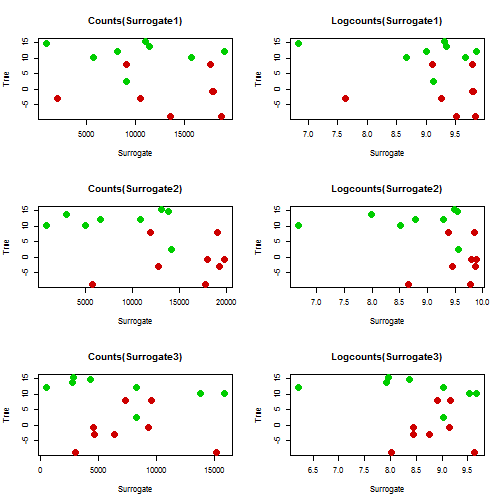
\includegraphics[scale=0.3]{first_presentation-figure/exploration-1.png}
%\caption{t}
\end{figure}
\end{minipage}
\hfill
\begin{minipage}{0.40\textwidth}
\begin{figure}[H]
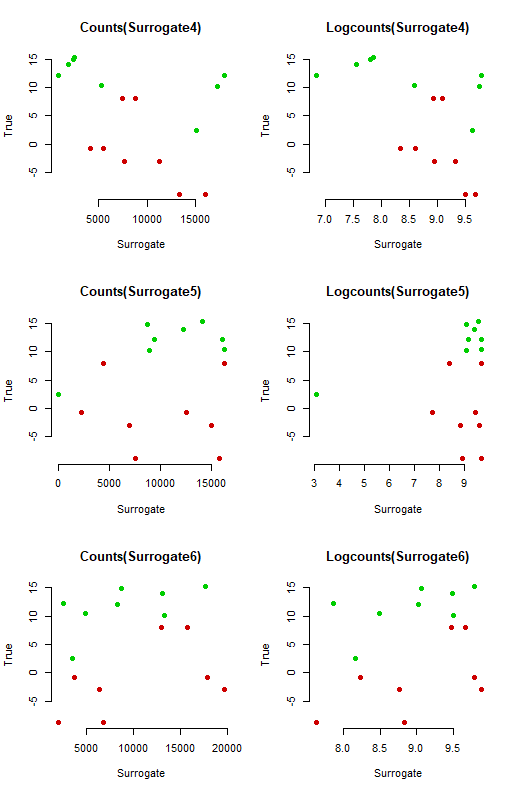
\includegraphics[scale=0.3]{first_presentation-figure/exploration-2.png}
%\caption{Wil}
\end{figure}

\end{minipage}

\begin{itemize}
\item red = control treatment, green = experimental treatment
\item y axis shows treatment effect on T
\item x axis shows treatment effect on S
\item the arrangement of the scattered points gives an idea of the adjusted association.
\end{itemize}

\end{frame}


\begin{frame}{Exploring Adjusted Association(cont:)}
\begin{minipage}{0.3\textwidth}
\begin{figure}[H]
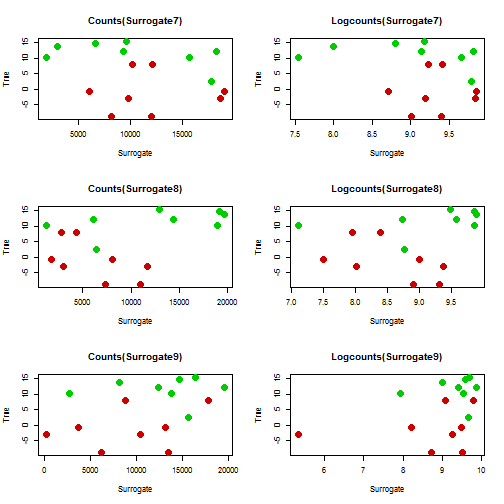
\includegraphics[scale=0.3]{first_presentation-figure/exploration-3.png}
%\caption{t}
\end{figure}
\end{minipage}
\hfill
\begin{minipage}{0.40\textwidth}
\begin{figure}[H]
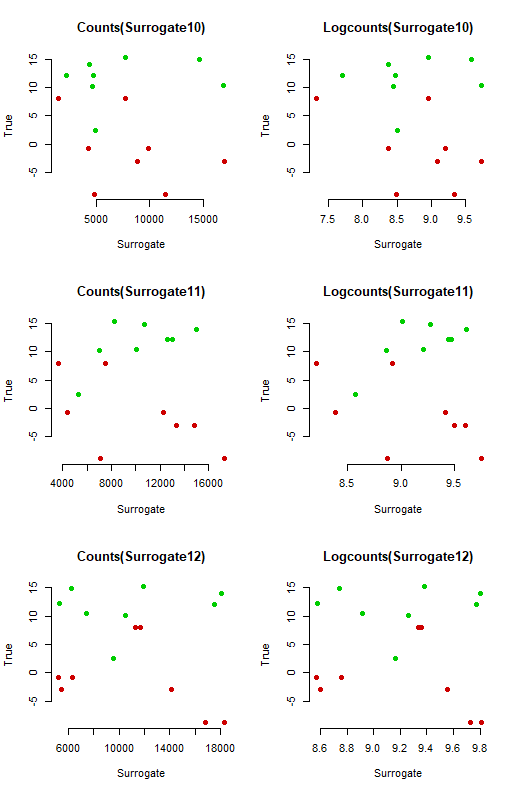
\includegraphics[scale=0.3]{first_presentation-figure/exploration-4.png}
%\caption{Wil}
\end{figure}

\end{minipage}

\end{frame}


\begin{frame}{Exploring Adjusted Association(cont:)}
\begin{minipage}{0.3\textwidth}
\begin{figure}[H]
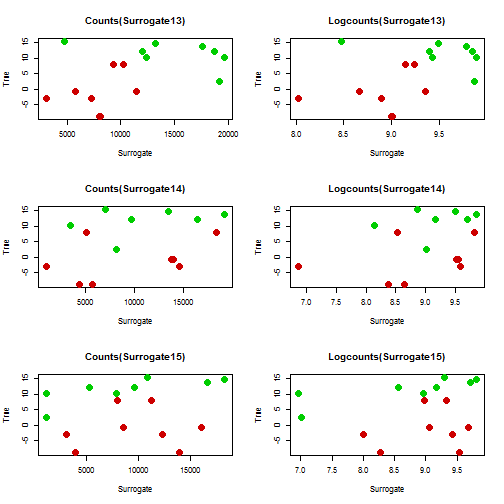
\includegraphics[scale=0.3]{first_presentation-figure/exploration-5.png}
%\caption{t}
\end{figure}
\end{minipage}
\hfill
\begin{minipage}{0.40\textwidth}
\begin{figure}[H]
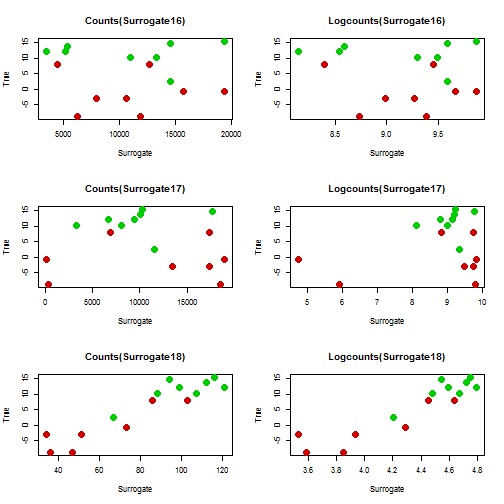
\includegraphics[scale=0.3]{first_presentation-figure/exploration-6.png}
%\caption{Wil}
\end{figure}

\end{minipage}
\end{frame}


\begin{frame}{Exploring Adjusted Association(cont:)}
\begin{minipage}{0.3\textwidth}
\begin{figure}[H]
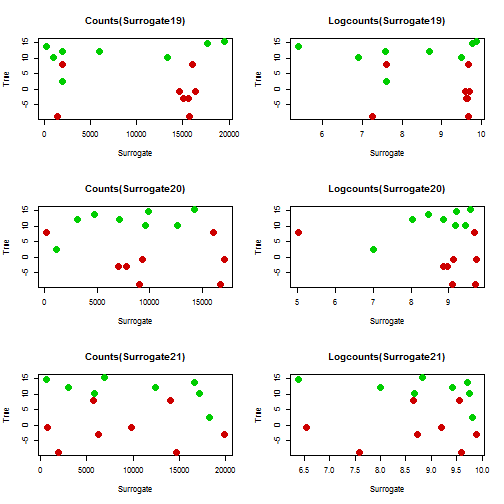
\includegraphics[scale=0.3]{first_presentation-figure/exploration-7.png}
%\caption{t}
\end{figure}
\end{minipage}
\hfill
\begin{minipage}{0.40\textwidth}
\begin{figure}[H]
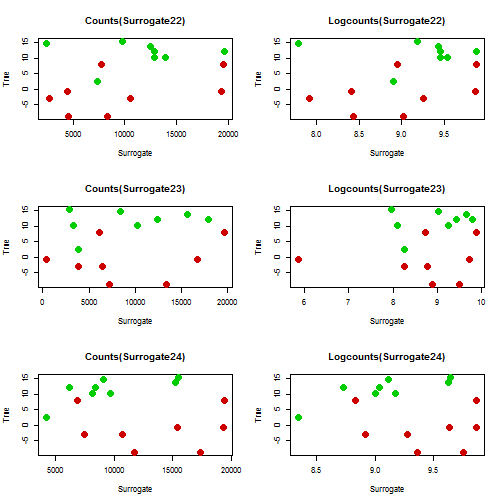
\includegraphics[scale=0.3]{first_presentation-figure/exploration-8.png}
%\caption{Wil}
\end{figure}
\end{minipage}
\end{frame}

\begin{frame}{Exploring Adjusted Association(cont:)}
\begin{minipage}{0.3\textwidth}
\begin{figure}[H]
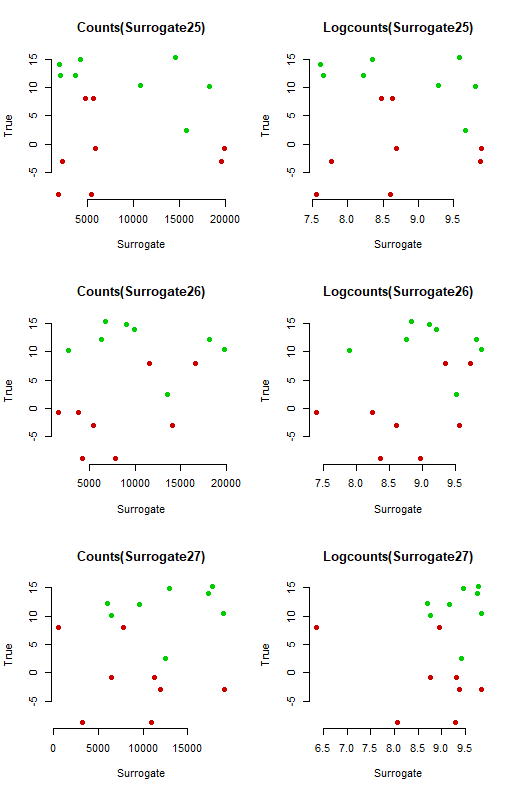
\includegraphics[scale=0.3]{first_presentation-figure/exploration-9.png}
%\caption{t}
\end{figure}
\end{minipage}
\hfill
\begin{minipage}{0.40\textwidth}
\begin{figure}[H]
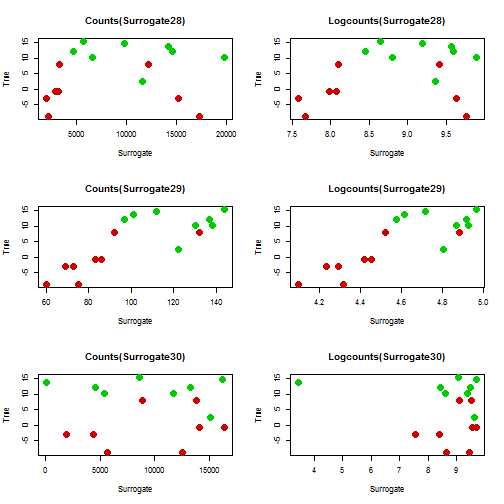
\includegraphics[scale=0.3]{first_presentation-figure/exploration-10.png}
%\caption{Wil}
\end{figure}
\end{minipage}
\end{frame}

\section{Results}
\subsection{Treatment Effects}

\begin{frame}{Treatment Effect on Insulin Sensitivity(T)}
A paired t-test and Wilcoxon test(due to the sample size) is used to test for treatmment effect on T. The null hypothesis of interest is; $$H_0: \mu_{T_c} = \mu_{T_E}$$

\begin{block}{t-test(treatment effect=difference in means)}
\begin{table}[H]
\begin{tabular}{cc}
\hline
Treatment Effect & 95\%CI\\
\hline
1257 & 6.68, 18.47\\
\hline
\end{tabular}
\end{table}
\end{block}

\begin{block}{Wilcoxon-test(treatment effect=difference in Ranks)}
\begin{table}[H]
\begin{tabular}{cc}
\hline
Treatment Effect & 95\%CI\\
\hline
1323 & 5.45, 18.96\\
\hline
\end{tabular}
\end{table}
\end{block}

\alert{Both tests showed a treatment effect in favor of the experimental treatment}.
\end{frame}

%\subsection{Surrogates}

\begin{frame}{Treatment Effect on Surrogates}
\alert{\textbf{Only the log of counts will be used from here onward.}}

The null hypothesis of interest remains; $$H_0: \mu_{S_C} = \mu_{S_E}$$ for each of the 30 surrogates.

\begin{minipage}{0.3\textwidth}
\begin{figure}[H]
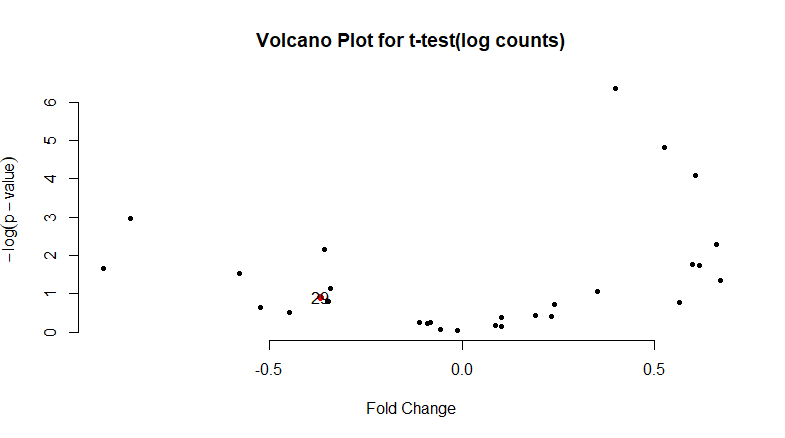
\includegraphics[scale=0.3]{t-testvolcano_plot_logcounts.png}
\caption{t-tests}
\end{figure}
\end{minipage}
\hfill
\begin{minipage}{0.5\textwidth}
\begin{figure}[H]
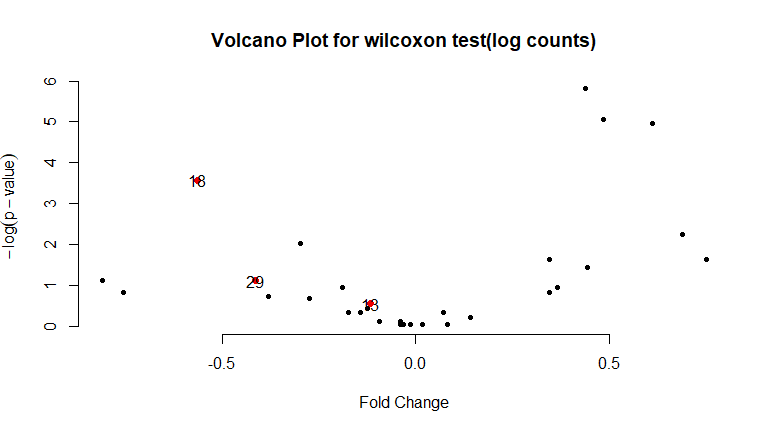
\includegraphics[scale=0.35]{wilcox_volcano_plot_logcounts.png}
\caption{Wilcoxon-tests}
\end{figure}

\end{minipage}
\end{frame}

\begin{frame}{Adjusted Treatment Effect on Surrogates}
\begin{table}[H]
\begin{minipage}{0.5\textwidth}
\centering
\begin{tabular}{rrrr}
  \hline
S & rawp & BH & fc \\ 
  \hline
  29 & 0.00 & 0.05 & -3272.38 \\ 
  18 & 0.01 & 0.12 & -7137.25 \\ 
  13 & 0.02 & 0.17 & -417.62 \\ 
  2 & 0.05 & 0.39 & -1358.12 \\ 
  28 & 0.10 & 0.57 & 632.38 \\ 
  24 & 0.11 & 0.57 & -1647.00 \\ 
  8 & 0.17 & 0.63 & -1749.12 \\ 
  27 & 0.18 & 0.63 & 6084.88 \\ 
  19 & 0.19 & 0.63 & 3720.62 \\ 
  4 & 0.21 & 0.64 & -674.75 \\ 
  9 & 0.26 & 0.70 & 186.50 \\ 
  7 & 0.32 & 0.80 & -328.88 \\ 
  26 & 0.34 & 0.80 & 6791.50 \\ 
  1 & 0.40 & 0.81 & 524.62 \\ 
  3 & 0.45 & 0.81 & -788.38 \\ 
  \hline
  \end{tabular}
\end{minipage}\hfill
\begin{minipage}{0.4\textwidth}
\begin{tabular}{rrrr}
\hline
S & rawp & BH & fc \\ 
  \hline
  15 & 0.45 & 0.81 & -295.00 \\ 
  17 & 0.47 & 0.81 & -1976.50 \\ 
  22 & 0.49 & 0.81 & 37.62 \\ 
  30 & 0.52 & 0.82 & -4382.62 \\
  5 & 0.61 & 0.88 & -2595.75 \\ 
  14 & 0.66 & 0.88 & 943.00 \\ 
  23 & 0.66 & 0.88 & 1754.12 \\ 
  11 & 0.68 & 0.88 & 106.88 \\ 
  6 & 0.77 & 0.92 & -3958.62 \\ 
  16 & 0.78 & 0.92 & 741.88 \\ 
  10 & 0.80 & 0.92 & 2626.62 \\ 
  25 & 0.85 & 0.92 & 3796.00 \\ 
  21 & 0.86 & 0.92 & 3601.38 \\ 
  20 & 0.93 & 0.96 & 38.88 \\ 
  12 & 0.96 & 0.96 & -346.50 \\ 
   \hline
\end{tabular}
\end{minipage}
\caption{t-tests}
\end{table}

\end{frame}

\begin{frame}{Adjusted Treatment Effect on Surrogates}
\begin{table}[H]
\centering
\begin{minipage}{0.5\textwidth}
\begin{tabular}{rrrrr}
  \hline
  S & rawp & BH & fc \\ 
  \hline
  29 & 0.00 & 0.07 & -3272.38 \\ 
  18 & 0.01 & 0.07 & -7137.25 \\ 
  13 & 0.01 & 0.07 & -417.62 \\ 
  2 & 0.03 & 0.21 & -1358.12 \\ 
  8 & 0.10 & 0.63 & 632.38 \\ 
  24 & 0.13 & 0.65 & -1647.00 \\ 
  9 & 0.19 & 0.73 & -1749.12 \\ 
  28 & 0.19 & 0.73 & 6084.88 \\ 
  27 & 0.23 & 0.78 & 3720.62 \\ 
  1 & 0.33 & 0.88 & -674.75 \\ 
  19 & 0.33 & 0.88 & 186.50 \\ 
  7 & 0.38 & 0.88 & -328.88 \\ 
  26 & 0.38 & 0.88 & 6791.50 \\ 
  4 & 0.44 & 0.88 & 524.62 \\ 
  22 & 0.44 & 0.88 & -788.38 \\ 
  \hline
  \end{tabular}
\end{minipage}\hfill
\begin{minipage}{0.4\textwidth}
\begin{tabular}{rrrr}
\hline
S & rawp & BH & fc \\ 
  \hline
  17 & 0.49 & 0.89 & -295.00 \\ 
  20 & 0.51 & 0.89 & -1976.50 \\ 
  3 & 0.57 & 0.96 & 37.62 \\ 
  10 & 0.65 & 0.96 & -4382.62 \\ 
  5 & 0.72 & 0.96 & -2595.75 \\ 
  6 & 0.72 & 0.96 & 943.00 \\ 
  15 & 0.72 & 0.96 & 1754.12 \\ 
  21 & 0.80 & 0.96 & 106.88 \\ 
  25 & 0.88 & 0.96 & -3958.62 \\ 
  30 & 0.88 & 0.96 & 741.88 \\ 
  11 & 0.96 & 0.96 & 2626.62 \\ 
  12 & 0.96 & 0.96 & 3796.00 \\ 
  14 & 0.96 & 0.96 & 3601.38 \\ 
  16 & 0.96 & 0.96 & 38.88 \\ 
  23 & 0.96 & 0.96 & -346.50 \\ 
   \hline
\end{tabular}
\end{minipage}
\caption{W-test} 
\end{table}

\end{frame}

\subsection{Joint Modelling}

\begin{frame}{Results from Joint Models}
\tiny
\begin{table}[ht]
\centering
\begin{tabular}{cccccccccc}
  \hline
$S_i$ & $\rho_{UN}$ & $\rho_{ADj}$ & LCI & UCI & $pval_{\rho}$ & $pval-adj_{\rho}$ & $\alpha_j$ & $pval_{\alpha_j}$ & $pval-adj_{\alpha_j}$ \\ 
  \hline
\alert{18} & 0.90 & 0.83 & 0.56 & 0.94 & 0.00 & 0.00 & 0.52 & 0.00 & 0.04 \\ 
 \alert{29} & 0.82 & 0.57 & 0.11 & 0.83 & 0.01 & 0.13 & 0.40 & 0.00 & 0.01\\ 
  \alert{6} & 0.29 & 0.56 & 0.10 & 0.83 & 0.01 & 0.13 & -0.11 & 0.77 & 0.92 \\ 
  \alert{15} & 0.12 & 0.46 & -0.05 & 0.78 & 0.05 & 0.36 & -0.35 & 0.44 & 0.80 \\ 
  \alert{5} & 0.14 & 0.41 & -0.11 & 0.75 & 0.09 & 0.44 & -0.45 & 0.60 & 0.88 \\ 
  \alert{14} & 0.29 & 0.32 & -0.21 & 0.70 & 0.19 & 0.74 & 0.19 & 0.65 & 0.88 \\ 
  \alert{24} & -0.18 & 0.25 & -0.28 & 0.67 & 0.30 & 0.82 & -0.36 & 0.10 & 0.52 \\ 
  \alert{22} & 0.29 & 0.23 & -0.30 & 0.65 & 0.35 & 0.82 & 0.24 & 0.48 & 0.80 \\ 
  \alert{17} & 0.27 & 0.19 & -0.34 & 0.63 & 0.44 & 0.82 & 0.56 & 0.45 & 0.80 \\ 
  \alert{26} & 0.31 & 0.19 & -0.34 & 0.62 & 0.45 & 0.82 & 0.35 & 0.34 & 0.78 \\ 
  9 & 0.33 & 0.15 & -0.37 & 0.60 & 0.55 & 0.82 & 0.67 & 0.24 & 0.65 \\ 
  23 & 0.17 & 0.12 & -0.40 & 0.58 & 0.62 & 0.82 & 0.23 & 0.66 & 0.88 \\ 
  2 & -0.34 & 0.10 & -0.42 & 0.57 & 0.69 & 0.82 & -0.86 & 0.03 & 0.26 \\ 
  19 & -0.22 & 0.10 & -0.42 & 0.56 & 0.70 & 0.82 & -0.93 & 0.17 & 0.58 \\ 
  13 & 0.44 & -0.04 & -0.52 & 0.47 & 0.88 & 0.88 & 0.61 & 0.01 & 0.11 \\ 
  28 & 0.31 & -0.05 & -0.53 & 0.46 & 0.84 & 0.87 & 0.66 & 0.08 & 0.51 \\ 
  30 & -0.18 & -0.06 & -0.54 & 0.45 & 0.80 & 0.86 & -0.52 & 0.51 & 0.80 \\ 
  25 & -0.01 & -0.08 & -0.55 & 0.43 & 0.75 & 0.84 & 0.09 & 0.85 & 0.92 \\ 
  1 & -0.23 & -0.09 & -0.56 & 0.42 & 0.71 & 0.82 & -0.37 & 0.40 & 0.80 \\ 
  8 & 0.22 & -0.10 & -0.56 & 0.42 & 0.70 & 0.82 & 0.60 & 0.16 & 0.58 \\ 
  21 & -0.03 & -0.11 & -0.58 & 0.41 & 0.65 & 0.82 & 0.10 & 0.86 & 0.92 \\ 
  16 & -0.13 & -0.12 & -0.58 & 0.40 & 0.64 & 0.82 & -0.08 & 0.77 & 0.92 \\ 
  3 & -0.23 & -0.12 & -0.58 & 0.40 & 0.64 & 0.82 & -0.35 & 0.43 & 0.80 \\ 
  7 & -0.29 & -0.13 & -0.59 & 0.39 & 0.59 & 0.82 & -0.34 & 0.31 & 0.77 \\ 
  12 & -0.10 & -0.14 & -0.59 & 0.38 & 0.58 & 0.82 & -0.01 & 0.96 & 0.96 \\ 
  20 & -0.14 & -0.19 & -0.63 & 0.34 & 0.45 & 0.82 & -0.06 & 0.93 & 0.96 \\ 
  11 & -0.05 & -0.22 & -0.64 & 0.31 & 0.38 & 0.82 & 0.10 & 0.67 & 0.88 \\ 
  10 & -0.20 & -0.24 & -0.66 & 0.29 & 0.34 & 0.82 & -0.09 & 0.80 & 0.92 \\ 
  27 & 0.10 & -0.31 & -0.70 & 0.22 & 0.20 & 0.74 & 0.62 & 0.16 & 0.58 \\ 
  4 & -0.52 & -0.44 & -0.77 & 0.07 & 0.06 & 0.36 & -0.58 & 0.19 & 0.58 \\ 
   \hline
\end{tabular}
%\caption{Ranked by Adjusted Association}
\end{table}

\begin{itemize}
\item pval=p-value, pval-adj=adjusted pvalue using BH, LCI-Lower Confidence Interval and UCI=Upper Confidence Interval for $\rho$ and results are ordered according to adjusted association.
\end{itemize}
\end{frame}

\subsection{Causal Inference Results}

\begin{frame}{Causal Inference Results}
\tiny

\begin{table}[ht]
\centering
\begin{tabular}{rrrrrrrrrr}
  \hline
S & $\rho_0$ & $LCI_0$ & $UCI_0$ & $\rho_1$ & $LCI_1$ & $UCI_1$ & ICA & LRan & URan \\ 
  \hline
 \alert{18} & 0.84 & 0.60 & 0.94 & 0.81 & 0.52 & 0.93 & 0.91 & -0.76 & 1.00 \\ 
    \alert{6} & 0.57 & 0.11 & 0.83 & 0.56 & 0.10 & 0.83 & 0.84 & -0.96 & 1.00 \\ 
   \alert{15} & 0.20 & -0.33 & 0.63 & 0.79 & 0.49 & 0.93 & 0.83 & -0.91 & 0.93 \\ 
   \alert{17} & 0.21 & -0.32 & 0.64 & 0.14 & -0.39 & 0.59 & 0.74 & -1.00 & 1.00 \\ 
   \alert{19} & 0.00 & -0.49 & 0.50 & 0.21 & -0.32 & 0.64 & 0.70 & -0.99 & 0.99 \\ 
   \alert{24} & -0.10 & -0.57 & 0.41 & 0.81 & 0.52 & 0.93 & 0.69 & -0.85 & 0.86 \\ 
   \alert{29} & 0.85 & 0.60 & 0.95 & -0.11 & -0.57 & 0.41 & 0.67 & -0.81 & 0.84 \\ 
   \alert{14} & 0.32 & -0.21 & 0.70 & 0.32 & -0.21 & 0.70 & 0.63 & -0.99 & 1.00 \\ 
    \alert{5} & -0.16 & -0.60 & 0.37 & 0.88 & 0.67 & 0.96 & 0.60 & -0.73 & 0.80 \\ 
   \alert{22} & 0.43 & -0.09 & 0.76 & -0.10 & -0.57 & 0.42 & 0.58 & -0.96 & 0.95 \\ 
    2 & 0.32 & -0.21 & 0.70 & -0.01 & -0.50 & 0.49 & 0.57 & -0.98 & 0.98 \\ 
   20 & -0.51 & -0.80 & -0.02 & 0.73 & 0.37 & 0.90 & 0.53 & -0.75 & 0.77 \\ 
   23 & 0.06 & -0.45 & 0.54 & 0.30 & -0.23 & 0.69 & 0.52 & -0.99 & 0.98 \\ 
    8 & -0.52 & -0.81 & -0.03 & 0.37 & -0.15 & 0.73 & 0.52 & -0.87 & 0.87 \\ 
   26 & 0.39 & -0.14 & 0.74 & -0.19 & -0.63 & 0.34 & 0.51 & -0.95 & 0.95 \\ 
   11 & -0.57 & -0.83 & -0.10 & 0.70 & 0.32 & 0.89 & 0.48 & -0.75 & 0.74 \\ 
    9 & 0.19 & -0.34 & 0.63 & 0.01 & -0.49 & 0.50 & 0.48 & -0.99 & 0.99 \\ 
    3 & 0.20 & -0.33 & 0.63 & -0.38 & -0.74 & 0.14 & 0.34 & -0.94 & 0.94 \\ 
   30 & 0.28 & -0.25 & 0.68 & -0.28 & -0.68 & 0.25 & 0.33 & -0.95 & 0.95 \\ 
   28 & 0.02 & -0.48 & 0.51 & -0.23 & -0.65 & 0.30 & 0.31 & -0.99 & 0.99 \\ 
    1 & 0.01 & -0.49 & 0.50 & -0.24 & -0.66 & 0.29 & 0.30 & -0.99 & 0.98 \\ 
   12 & -0.27 & -0.67 & 0.26 & 0.09 & -0.43 & 0.56 & 0.28 & -0.97 & 0.98 \\ 
   13 & 0.29 & -0.24 & 0.69 & -0.50 & -0.80 & -0.00 & 0.17 & -0.91 & 0.90 \\ 
    7 & 0.06 & -0.45 & 0.54 & -0.32 & -0.70 & 0.21 & 0.14 & -0.98 & 0.97 \\ 
   16 & -0.10 & -0.57 & 0.42 & -0.15 & -0.60 & 0.37 & 0.13 & -0.99 & 0.99 \\ 
   25 & 0.18 & -0.34 & 0.62 & -0.47 & -0.78 & 0.04 & 0.05 & -0.93 & 0.93 \\ 
   27 & -0.44 & -0.77 & 0.07 & 0.16 & -0.37 & 0.61 & 0.05 & -0.95 & 0.95 \\ 
   10 & -0.48 & -0.79 & 0.02 & 0.18 & -0.35 & 0.62 & 0.05 & -0.93 & 0.94 \\ 
   21 & 0.12 & -0.40 & 0.58 & -0.47 & -0.78 & 0.03 & 0.03 & -0.95 & 0.94 \\ 
    4 & -0.49 & -0.79 & 0.01 & -0.59 & -0.84 & -0.13 & -0.79 & -1.00 & 0.97 \\ 
   \hline
\end{tabular}
\caption{Ranked by ICA values}
\end{table}

\end{frame}


\begin{frame}{Distribution of ICA}
\begin{minipage}{0.3\textwidth}
\begin{figure}[H]
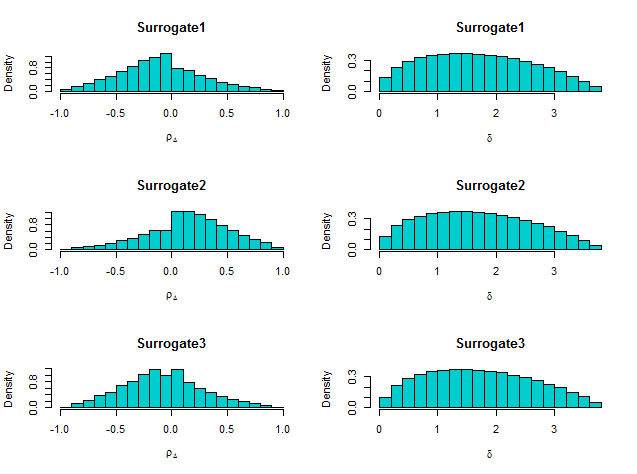
\includegraphics[scale=0.32]{icaplots1.png}
%\caption{t}
\end{figure}
\end{minipage}
\hfill
\begin{minipage}{0.40\textwidth}
\begin{figure}[H]
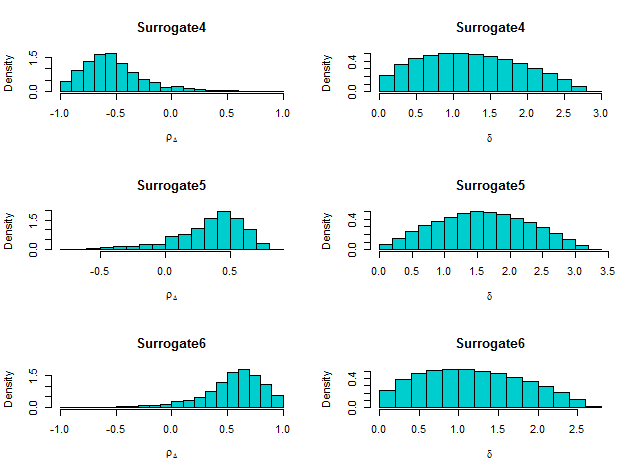
\includegraphics[scale=0.32]{icaplots2.png}
%\caption{Wil}
\end{figure}

\end{minipage}

%\begin{itemize}
%\item red = control treatment, green = experimental treatment
%\item y axis shows treatment effect on T
%\item x axis shows treatment effect on S
%\item the arrangement of the scattered points gives an idea of the adjusted association.
%\end{itemize}

\end{frame}


\begin{frame}{Distribution of ICA(cont:)}
\begin{minipage}{0.3\textwidth}
\begin{figure}[H]
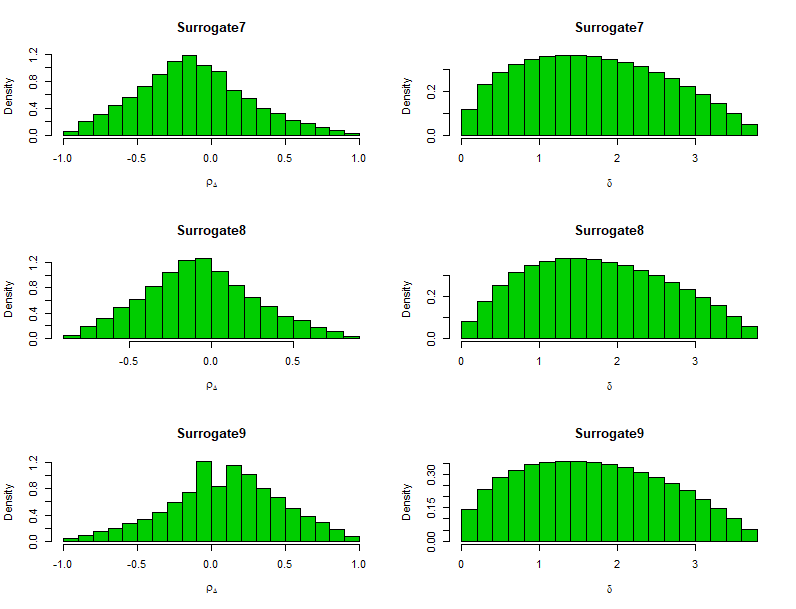
\includegraphics[scale=0.32]{icaplots3.png}
%\caption{t}
\end{figure}
\end{minipage}
\hfill
\begin{minipage}{0.40\textwidth}
\begin{figure}[H]
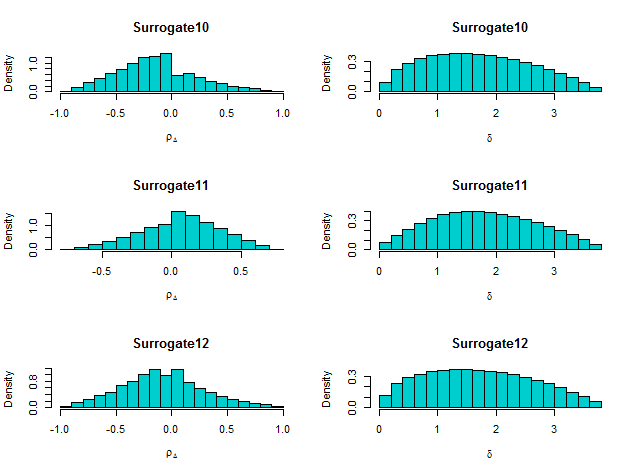
\includegraphics[scale=0.32]{icaplots4.png}
%\caption{Wil}
\end{figure}

\end{minipage}

\end{frame}


\begin{frame}{Distribution of ICA(cont:)}
\begin{minipage}{0.3\textwidth}
\begin{figure}[H]
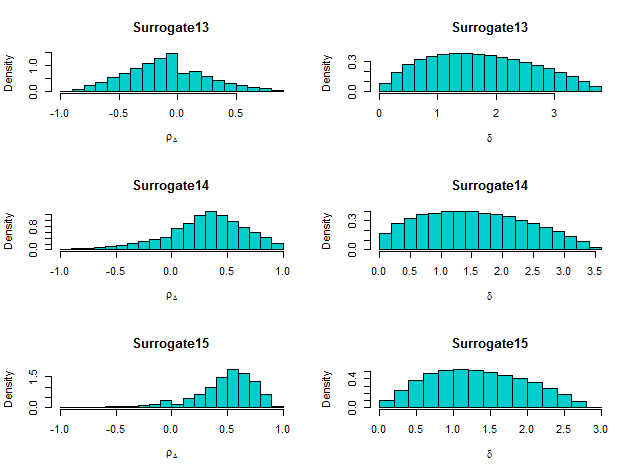
\includegraphics[scale=0.32]{icaplots5.png}
%\caption{t}
\end{figure}
\end{minipage}
\hfill
\begin{minipage}{0.40\textwidth}
\begin{figure}[H]
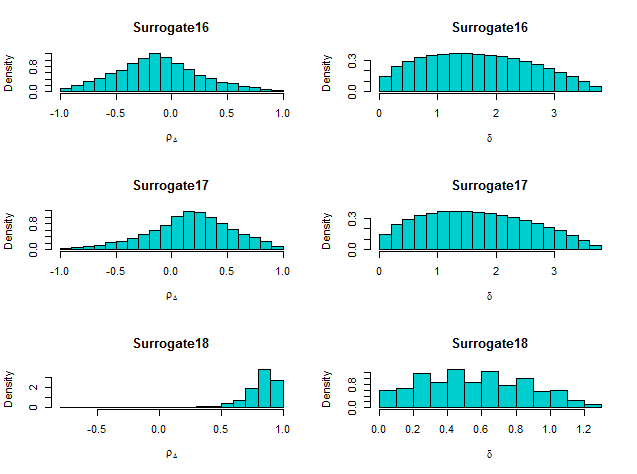
\includegraphics[scale=0.32]{icaplots6.png}
%\caption{Wil}
\end{figure}

\end{minipage}
\end{frame}


\begin{frame}{Distribution of ICA(cont:)}
\begin{minipage}{0.3\textwidth}
\begin{figure}[H]
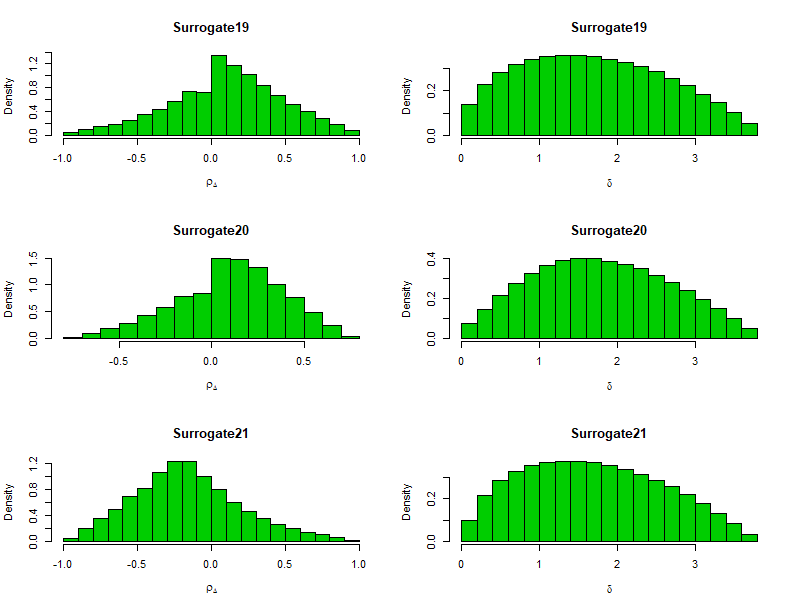
\includegraphics[scale=0.32]{icaplots7.png}
%\caption{t}
\end{figure}
\end{minipage}
\hfill
\begin{minipage}{0.40\textwidth}
\begin{figure}[H]
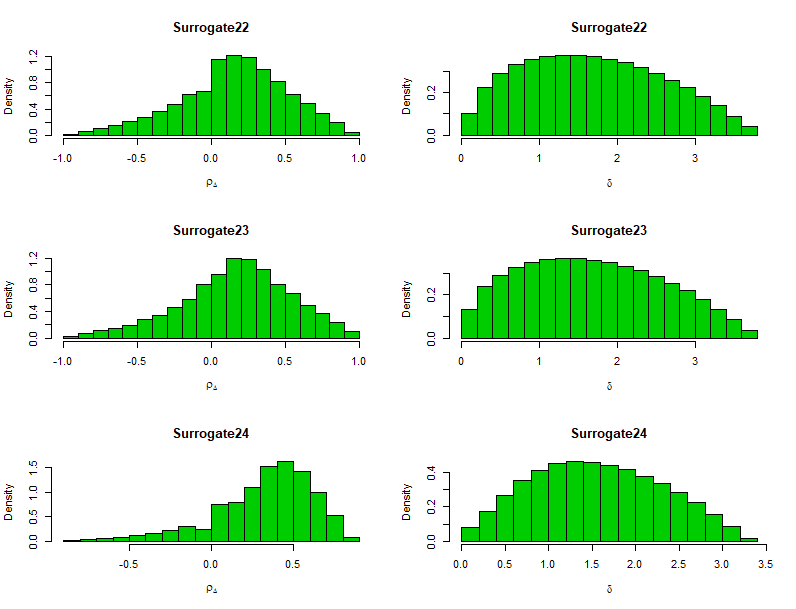
\includegraphics[scale=0.32]{icaplots8.png}
%\caption{Wil}
\end{figure}
\end{minipage}
\end{frame}

\begin{frame}{Distribution of ICA(cont:)}
\begin{minipage}{0.3\textwidth}
\begin{figure}[H]
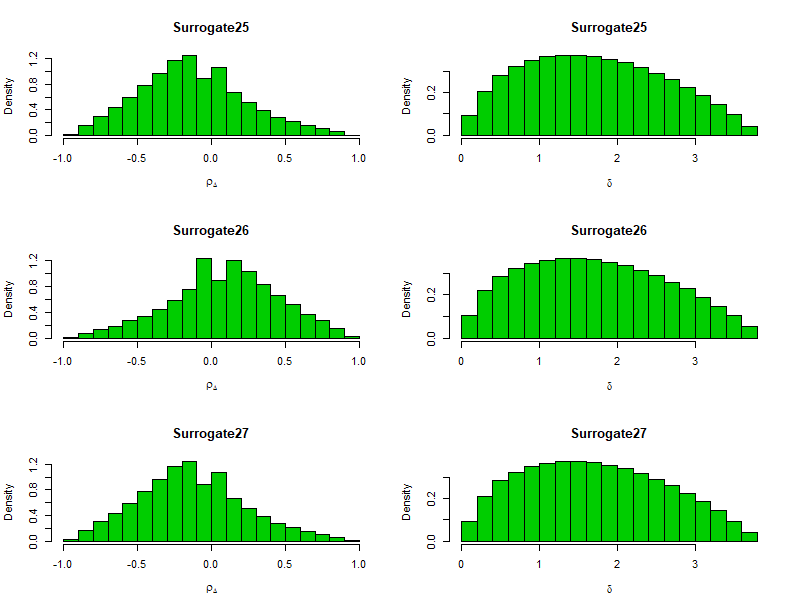
\includegraphics[scale=0.32]{icaplots9.png}
%\caption{t}
\end{figure}
\end{minipage}
\hfill
\begin{minipage}{0.40\textwidth}
\begin{figure}[H]
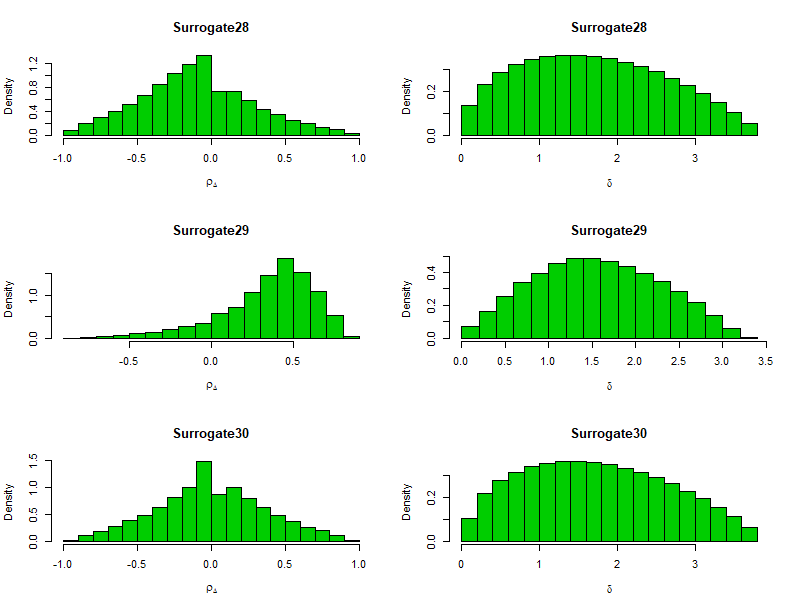
\includegraphics[scale=0.32]{icaplots10.png}
%\caption{Wil}
\end{figure}
\end{minipage}
\end{frame}

\section{Discussion of Results}

\begin{frame}{What We Learn from The Results}
\begin{itemize}
\item The exploration revealed the possibility of high adjusted association between surrogate 29, 18 and T.
\item The joint model confirmed the suspicion of high adjusted association$(\rho_{T,S|X} = 0.83)$ between 18 and T. The obtained ICA for this surrogate is also high $(\rho_{\Delta} = 0.91)$ but the range of obtained ICA values is quite large (-0.76, 1) but in most cases, these ICA values are larger than 0.7(see ICA distribution for surrogate 18).

\item The adjusted association for surrogate 29 was a moderate association $(\rho_{T,S|X} = 0.57)$. Results from the causal inference framework showed that the relationship between T and surrogate 29 is opposite in the treatment groups ($\rho_0 = 0.85, \rho_1 = -0.11$). This is potentially responsible for the moderate adjusted association,

\item Studying the top 10 surrogates in each approach showed that only surrogate 19 made it to the top 10 in CIA that was not present in the JMA, while only surrogate 26 made it in JMA and is not present in CIA. Notably, surrogate 26 had opposite relationship between T and S in the treatment groups ($\rho_0 = 0.39, \rho_1 = -0.19$).

\end{itemize}
\end{frame}


\end{document}
